\documentclass[10pt,a4paper]{beamer}
\usetheme{Malmoe}
\definecolor{UniGreen}{RGB}{0,150,0}
\setbeamercolor{title}{fg=UniGreen}
\setbeamercolor{frametitle}{fg=UniGreen}
\setbeamercolor{structure}{fg=UniGreen}
\usepackage[utf8]{inputenc}
\usepackage[MeX]{polski}
\usepackage{amsmath}
\usepackage{amsfonts}
\usepackage{amssymb}
\usepackage{graphicx}
\usepackage{rotating}
\usepackage{multirow}
\author{\texorpdfstring{Jakub Turek \newline \href{mailto:jkbturek@gmail.com}{ jkbturek@gmail.com }}{Jakub Turek}}
\title{Komputerowy gracz Scrabble}
\institute{Wydział Elektroniki i Technik Informacyjnych}
\begin{document}

\begin{frame}
	\titlepage
\end{frame}

\section{Wstęp}

\begin{frame}
	\frametitle{Historia Scrabble}
	
	\begin{itemize}
		\item 1938 r. - gra \emph{Lexiko}, Alfred Mosher Butts.
		\item \emph{Criss-Crossword} - udoskonalona wersja \emph{Lexiko}.
		\item 1948 r. - James Burnot, \emph{Scrabble}.
		\item Lata 80. - Hasbro.
		\item ,,Bohater'' teleturnieju \emph{Scrabble}.
		\item 121 krajów, 29 różnych języków.
		\item 150 milionów sprzedanych egzemplarzy.
	\end{itemize}
\end{frame}

\subsection{Zasady}

\begin{frame}
	\frametitle{Plansza}
	
	\begin{columns}[onlytextwidth]
		\begin{column}{0.55\textwidth}
			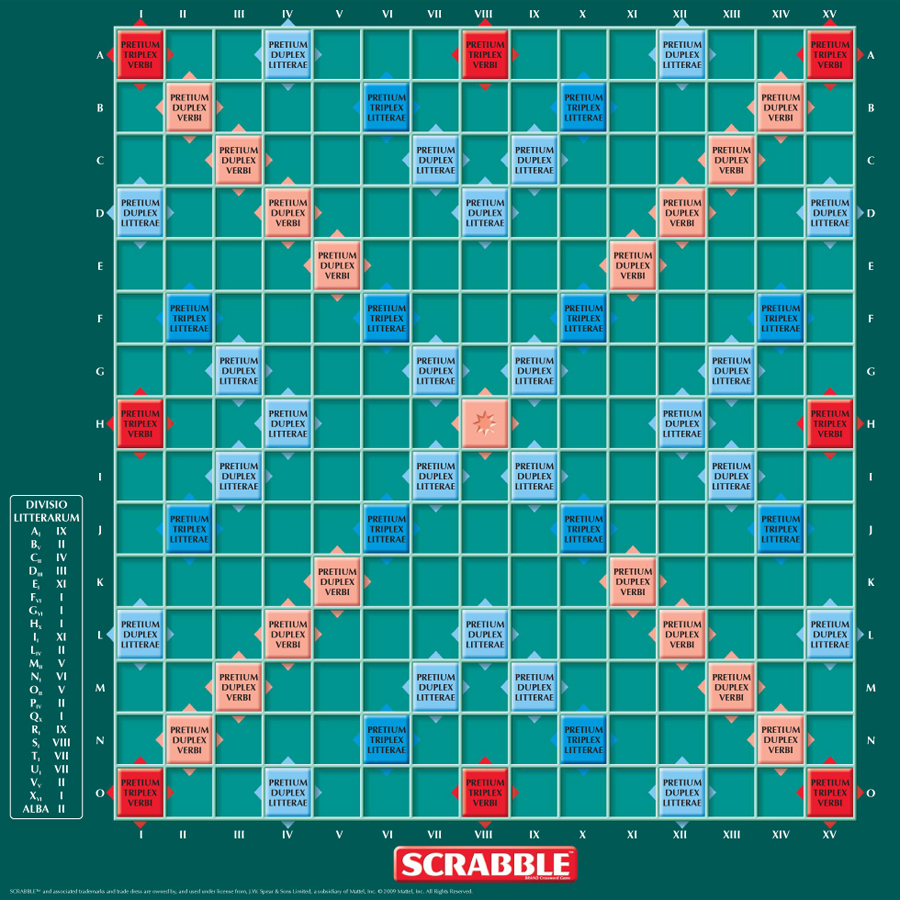
\includegraphics[scale=0.17]{graphics/board.jpg}
		\end{column}
		\begin{column}{0.45\textwidth}
			\begin{itemize}
				\item Wymiary $15 \times 15$.
				\item Premie:
					\begin{itemize}
						\item literowe:
							\begin{itemize}
								\item podwójna,
								\item potrójna.
							\end{itemize}
						\item słowne:
							\begin{itemize}
								\item podwójna,
								\item potrójna.
							\end{itemize}
					\end{itemize}
				\item Środek planszy:
					\begin{itemize}
						\item pierwszy wyraz musi przechodzić przez pole,
						\item podwójna premia słowna.
					\end{itemize}
			\end{itemize}
		\end{column}
	\end{columns}
\end{frame}

\begin{frame}
	\frametitle{Płytki (polska wersja)}
	
	\begin{columns}[onlytextwidth]
		\begin{column}{0.55\textwidth}
			\scalebox{0.8}{
				\begin{tabular}{|c|c|c||c|c|c||c|c|c|}
					\hline
					\multirow{16}{*}{
						\begin{sideways}
							Litera
						\end{sideways}	} &
					\multirow{16}{*}{
						\begin{sideways}
							Ilość płytek
						\end{sideways}} & 
					\multirow{16}{*}{
						\begin{sideways}
							Liczba punktów
						\end{sideways}} & \textbf{A} & 9 & 1 & \textbf{M} & 3 & 2 \\
					\cline{4-9}
					&&& \textbf{Ą} & 1 & 5 & \textbf{N} & 5 & 1 \\
					\cline{4-9}
					&&& \textbf{B} & 2 & 3 & \textbf{Ń} & 1 & 7 \\			
					\cline{4-9}
					&&& \textbf{C} & 3 & 2 & \textbf{O} & 6 & 1 \\			
					\cline{4-9}
					&&& \textbf{Ć} & 1 & 6 & \textbf{Ó} & 1 & 5 \\
					\cline{4-9}
					&&& \textbf{D} & 3 & 2 & \textbf{P} & 3 & 2 \\	
					\cline{4-9}
					&&& \textbf{E} & 7 & 1 & \textbf{R} & 4 & 1 \\
					\cline{4-9}
					&&& \textbf{Ę} & 1 & 5 & \textbf{S} & 4 & 1 \\
					\cline{4-9}
					&&& \textbf{F} & 1 & 5 & \textbf{Ś} & 1 & 5 \\
					\cline{4-9}				
					&&& \textbf{G} & 2 & 3 & \textbf{T} & 3 & 2 \\
					\cline{4-9}
					&&& \textbf{H} & 2 & 3 & \textbf{U} & 2 & 3 \\
					\cline{4-9}
					&&& \textbf{I} & 8 & 1 & \textbf{W} & 4 & 1 \\
					\cline{4-9}
					&&& \textbf{J} & 2 & 3 & \textbf{Y} & 4 & 2 \\
					\cline{4-9}
					&&& \textbf{K} & 3 & 2 & \textbf{Z} & 5 & 1 \\
					\cline{4-9}
					&&& \textbf{L} & 3 & 2 & \textbf{Ź} & 1 & 9 \\
					\cline{4-9}
					&&& \textbf{Ł} & 2 & 3 & \textbf{Ż} & 1 & 5 \\
					\hline
				\end{tabular}
			}
		\end{column}
		\begin{column}{0.45\textwidth}
			\begin{itemize}
				\item 98 płytek z~literami.
				\item Każda litera ma przyporządkowaną punktację.
				\item Ilość płytek proporcjonalna do częstotliwości występowania litery.
				\item Punktacja odwrotnie proporcjonalna do częstotliwości występowania litery.
				\item 2 \emph{blanki}.
			\end{itemize}
		\end{column}
	\end{columns}
\end{frame}

\begin{frame}
	\frametitle{Reguły}
	
	\begin{itemize}
		\item Na stojaku 7 wylosowanych płytek.
		\item Naprzemienne ruchy.
		\item Prawidłowy ruch:
			\begin{itemize}
				\item Płytki wyłożone w~jednym wierszu (lub kolumnie) w~sposób ciągły.
				\item Wykorzystanie przynajmniej jednej litery znajdującej się już na planszy.
				\item Tworzy poprawny wyraz czytany od lewej do prawej (lub od góry do dołu).
				\item Wszystkie płytki przylegające tworzą poprawne wyrazy w~układzie krzyżówkowym.
			\end{itemize}
		\item Koniec gry - pierwszy gracz, który nie ma płytek na stojaku.
		\item Wygrywa gracz z~największą liczbą punktów.
	\end{itemize}
\end{frame}

\begin{frame}
	\frametitle{Dopuszczalne słowa}
	
	Dopuszczalne jest wykorzystanie wszystkich słów znajdujących się w~dowolnym słowniku języka polskiego (wraz z~poprawnymi odmianami) z~wyłączeniem:
	
	\begin{itemize}
		\item nazw własnych (wyrazów pisanych z~wielkiej litery),
		\item skrótów,
		\item przedrostków, przyrostków,
		\item wyrazów wymagających użycia apostrofu lub łącznika.
	\end{itemize}
\end{frame}

\end{document}